%==============================================================================
% Sjabloon onderzoeksvoorstel bachproef
%==============================================================================
% Gebaseerd op document class `hogent-article'
% zie <https://github.com/HoGentTIN/latex-hogent-article>

% Voor een voorstel in het Engels: voeg de documentclass-optie [english] toe.
% Let op: kan enkel na toestemming van de bachelorproefcoördinator!
\documentclass{hogent-article}
\usepackage{tikz}
\usetikzlibrary{shapes.geometric, arrows}
\tikzstyle{startstop} = [rectangle, rounded corners, minimum width=3cm, minimum height=1cm,text centered, draw=black, fill=red!30]
\tikzstyle{io} = [trapezium, trapezium left angle=70, trapezium right angle=110, minimum width=3cm, minimum height=1cm, text centered, draw=black, fill=blue!30]
\tikzstyle{process} = [rectangle, minimum width=3cm, minimum height=1cm, text centered, draw=black, fill=orange!30]
\tikzstyle{decision} = [diamond, minimum width=3cm, minimum height=1cm, text centered, draw=black, fill=green!30]
\tikzstyle{arrow} = [thick,->,>=stealth]
\tikzstyle{process} = [rectangle, minimum width=3cm, minimum height=1cm, text centered, text width=3cm, draw=black, fill=orange!30]
% Invoegen bibliografiebestand
\addbibresource{voorstel.bib}

% Informatie over de opleiding, het vak en soort opdracht
\studyprogramme{Professionele bachelor toegepaste informatica}
\course{Bachelorproef}
\assignmenttype{Onderzoeksvoorstel}
% Voor een voorstel in het Engels, haal de volgende 3 regels uit commentaar
% \studyprogramme{Bachelor of applied information technology}
% \course{Bachelor thesis}
% \assignmenttype{Research proposal}

\academicyear{2023-2024} % TODO: pas het academiejaar aan

% TODO: Werktitel
\title{Het lokaal uitvoeren van Machine Learning pipelines: een vergelijkende studie en proof of concept.}

% TODO: Studentnaam en emailadres invullen
\author{Casper Audenaert}
\email{casper.audenaert@student.hogent.be}

% TODO: Geef de co-promotor op
\supervisor[Co-promotor]{T. Aelbrecht (HoGent, \href{mailto:thomas.aelbrecht@hogent.be}{thomas.aelbrecht@hogent.be})}

% Binnen welke specialisatierichting uit 3TI situeert dit onderzoek zich?
% Kies uit deze lijst:
%
% - Mobile \& Enterprise development
% - AI \& Data Engineering
% - Functional \& Business Analysis
% - System \& Network Administrator
% - Mainframe Expert
% - Als het onderzoek niet past binnen een van deze domeinen specifieer je deze
%   zelf
%
\specialisation{AI \& Data Engineering}
\keywords{cloud, CI/CD pipelines, machine learning operations, Kubeflow}

\begin{document}

\begin{abstract}
  Dit onderzoeksvoorstel richt zich op het verkennen van de mogelijkheden voor het lokaal uitvoeren van machine learning pipelines, met een focus of Kubeflow en alternatieve frameworks.
  Binnen het keuzepakket ``AI \& Data Engineering'' en het bijbehorende opleidingsonderdeel ``Machine Learning Operations'' wordt er momenteel gebruikgemaakt van Azure ML pipelines voor het uitvoeren van machine learning in de Azure Cloud.
  Het gebruik van Azure ML pipelines is namelijk niet gratis voor studenten die niet genoeg krediet hebben op het platform. Hierdoor richt dit onderzoek zich op het lokaal uitvoeren van machine learning pipelines.
  De basis van Azure ML pipelines is Kubeflow. Voor het lokaal draaien van Kubeflow zijn er echter aanzienlijke uitdagingen, waardoor het noodzakelijk is om een aangepaste Proof of Concept (PoC) op te stellen.
  Het lokaal uitvoeren van machine learning pipelines kan ook problemen met zich meebrengen, zoals de noodzaak van veel rekenkracht die mogelijk niet beschikbaar is op lokale computers. Als gevolg daarvan hebben bepaalde frameworks een beperkte versie die niet zo krachtig is als de cloud, maar toch lokaal machine learning pipelines kan uitvoeren.
  De eerste fase van deze bachelorproef omvat een diepgaande literatuurstudie, waarin wordt onderzocht welke frameworks bestaan voor het lokaal draaien van machine learning pipelines, hoe deze frameworks functioneren, en ook de compatibiliteit en diverse functies ervan.
  Het tweede deel van dit onderzoek richt zich op het opzetten van een Proof of Concept voor de geselecteerde tool(s), mogelijks vertrekkende van publiek beschikbare manifest bestanden. Hierbij wordt specifiek aandacht besteed aan het gemak van onderhoud voor de betrokken lectoren.
  Het verwachte resultaat van deze studie is een diepgaand inzicht in de geschiktheid van verschillende frameworks voor het lokaal uitvoeren van machine learning pipelines, met praktische toepasbaarheid in het onderwijs en het bedrijfsleven.
\end{abstract}

\tableofcontents

% De hoofdtekst van het voorstel zit in een apart bestand, zodat het makkelijk
% kan opgenomen worden in de bijlagen van de bachelorproef zelf.
%---------- Inleiding ---------------------------------------------------------

\section{Introductie}%
\label{sec:introductie}

De toename van Artificiële Intelligentie (AI), Machine Learning (ML) en Deep Learning heeft geleid tot een groeiende vraag naar manieren om Machine Learning modellen op een schaalbare en efficiënte manier te implementeren en te beheren \autocite{Aggarwal2022}.
Binnen het keuzepakket ``AI \& Data Engineering'' right het opleidingsonderdeel ``Machine Learning Operations'' zich op het opzetten van machine learning werkruimtes en het monitoren van machine learning operaties. In dit vak leert de student complexe IT-oplossingen efficiënt en zelfstandig te installeren, configureren, beveiligen, onderhouden en aanpassen, zodat ze blijven voldoen aan de veranderende behoeften. De student leert ook de CI/CD-principes toe te passen binnen de context van machine learning, zoals het beschrijven van deze principes, het in productie brengen en monitoren van een machine learning model met behulp van CI/CD-principes. Verder kan de student de uitdagingen en mogelijke oplossingen beschrijven voor het draaien van een machine learning model op apparaten met beperkte rekenkracht, en het model laten werken op zo'n apparaat, bijvoorbeeld door gebruik te maken van TensorFlow Lite.
Dit onderzoek richt zich op een specifieke uitdaging binnen Machine Learning Operations: het lokaal uitvoeren van Machine Learning pipelines.

In het kader van dit opleidingsonderdeel wordt er gebruik gemaakt van Azure ML pipelines, waarvan het onderliggende framework Kubeflow is. Kubeflow is een open-source Machine Learning toolkit op Kubernetes \autocite{Kubeflow2021}.
Het gebruik van Azure ML pipelines is namelijk niet gratis voor studenten die niet genoeg krediet hebben op het platform. Dit leidt ertoe dat dit onderzoek zich richt op het lokaal uitvoeren van machine learning pipelines.
Het lokaal uitvoeren van Machine Learning pipelines kan ook problemen met zich meebrengen, zoals de noodzaak van veel rekenkracht die mogelijk niet beschikbaar is op computers van studenten. Als gevolg daarvan hebben bepaalde frameworks een beperkte versie die niet zo krachtig is als de cloud-variant, maar toch lokaal Machine Learning pipelines kan uitvoeren.
Er zal onderzoek gedaan worden naar alternatieve frameworks om Machine Learning pipelines lokaal uit te voeren. Deze zullen met elkaar worden vergeleken om vervolgens een Proof of Concept (PoC) op te stellen. Hierbij zal gekeken worden naar hoe de verschillende frameworks en bibliotheken werken, welke programmeertaal ze gebruiken en welke functies ze aanbieden. Daarnaast worden de frameworks getest op de compatibiliteit met verschillende besturingssystemen. Deze test omvat gedetailleerde installaties van alle frameworks, waarvan de resultaten worden vastgelegd in een rapport.

Dit onderzoek richt zich op IT-professionals die betrokken zijn bij Machine Learning Operations, specifiek voor de diegenen die ML-pipelines lokaal willen uitvoeren.
Het lokaal uitvoeren van Machine Learning pipelines blijkt een uitdaging te zijn, vooral met betrekking tot de huidige migratieproblemen en gebrekkige documentatie.
De centrale onderzoeksvraag is daarom: ``Hoe kan een ML-pipeline lokaal worden uitgevoerd met behulp van een Machine Learning framework?''
Hierbij worden de volgende deelvragen behandeld:
\begin{itemize}
  \item Wat zijn de belangrijkste uitdagingen bij het lokaliseren van Machine Learning pipelines?
  \item Welke specifieke problemen kunnen optreden bij het lokaal uitvoeren van Machine\\ Learning pipelines?
  \item Hoe vertaalt de lokale uitvoering van een ML pipeline zich naar de cloud?
  \item Wat zijn de hardware- en softwarevereisten voor het lokaal uitvoeren van een ML-pipeline?
  \item Welke frameworks en tools kunnen worden gebruikt om Machine Learning pipelines lokaal uit te voeren, en wat zijn hun respectieve kenmerken en voordelen?
\end{itemize}


%---------- Stand van zaken ---------------------------------------------------

\section{Literatuurstudie}%
\label{sec:state-of-the-art}

De exponentiële groei van Machine Learning heeft niet alleen het onderzoeksdomein beïnvloed, maar heeft de implementatie van Machine Learning pipelines tot leven gebracht \autocite{Aggarwal2022}.
Deze literatuurstudie werpt een diepgaande blik op het lokaal uitvoeren van Machine Learning pipelines.
De focus van deze literatuurstudie zal liggen op de fundamentele elementen van Machine Learning pipelines, zoals de definitie van Machine Learning en pipelines, evenals een overzicht van de beschikbare frameworks voor het lokale uitvoeren van Machine Learning pipelines.
\subsection{Machine Learning}
Machine Learning (ML) is een onderliggend deel van Artificiële Intelligentie (AI), een snel groeiend vakgebied op het raakvlak van data en statistiek dat feitgebaseerde beslissingen in verschillende sectoren aanstuurt \autocite{Jordan2015}.
Middels het toepassen van wiskundige principes kan Machine Learning verbanden leggen tussen gegevens om betrouwbare voorspellingen te genereren. Dit wordt mogelijk gemaakt door het gebruik van Machine Learning algoritmen, waarmee computers kunnen leren van data. Met gebruik van iteratieve testen en validatie kunnen ze hun prestaties in de loop van de tijd verbeteren, waardoor ze nieuwe taken kunnen uitvoeren met nieuwe data \autocite{Shaveta2023}.
\subsection{CI/CD pipelines}
Een Continuous Integration/Continuous Deployment (CI/CD) pipeline vormt een cruciaal onderdeel van moderne softwareontwikkeling, gericht op het versnellen en betrouwbaarder maken van de levering van webapplicaties \autocite{Singh2023}. Deployment binnen de pipeline verwijst naar het proces van het implementeren van nieuwe code of updates naar de productieomgeving, terwijl delivery verwijst naar het proces van het gereed maken van nieuwe code of updates voor implementatie. De effectiviteit van deze pipelines is sterk afhankelijk van regelmatig onderhoud en updates om gelijke tred te houden met veranderingen in systemen en technologieën. Binnen het domein van datamanagement benadrukken \textcite{Samad2018} en \textcite{Vadavalasa2020} respectievelijk de cruciale aspecten van het optimaliseren van beperkte datasets en de implementatie van Continuous Integration in de datapipeline. Deze inzichten vormen de kern van een intrigerend verhaal dat draait om de zoektocht naar efficiëntie en effectiviteit bij het omgaan met gegevens. In deze studies wordt ook aangetoond dat het verzamelen van data veel geld kan kosten en veel tijd in beslag kan nemen. Verder tonen deze studies aan dat nauwkeurige modellen kunnen worden gegenereerd met behulp van ML-pipelines en een beperkte dataset. Dit onderzoeksvoorstel benadrukt ook de bijdragen van \textcite{Zhang2022} als belangrijke figuren met hun eigen inzichten.
\textcite{Zhang2022} richten zich op het ontwerpen en automatiseren van datapipelines. Hij toont aan dat met behulp van datapipelines dat een Machine Learning model veel efficiënter kan worden getraind, omdat de data goed wordt schoongemaakt en verwerkt, zodat onnodige of ontbrekende data niet de accuraatheid van het model beïnvloedt.
\subsection{Machine Learning frameworks en libraries}
De ontwikkeling van Machine Learning (ML) frameworks en bibliotheken heeft in de afgelopen 25 jaar een aanzienlijke vooruitgang gekend \autocite{Nguyen2019}. Deze tools hebben als gemeenschappelijk doel om de complexe\newline data-analyseprocessen te vergemakkelijken en geïntegreerde omgevingen te bieden bovenop standaard programmeertalen. Ze zijn ontworpen voor diverse doeleinden, variërend van analytische platformen, voorspellende systemen tot aanbevelingssystemen en verwerkingstools voor beeld-, geluids- of taaldata. Sommige zijn gericht op snelle verwerking en streaming van grootschalige data, terwijl andere gespecialiseerd zijn in het implementeren van ML-algoritmen, waaronder Neurale Netwerken (NNs) en Deep Learning (DL). Het is belangrijk om te benadrukken dat er geen enkele tool is die geschikt is voor elk probleem, en vaak is een combinatie van tools nodig om succesvol te zijn.

\subsubsection{Kubeflow}
\textcite{Kubeflow2021} is een open-source platform dat een collectie van Machine Learning tools biedt die compatibel zijn met Kubernetes. Het wordt vooral gebruikt in DevOps-frameworks, waar het Machine Learning stacks en componenten zoals PyTorch en TensorFlow kan beheren \autocite{Chandana2021}.

Kubeflow kan ook gebruikt worden bij end-to-end Machine Learning oplossingen, waarbij pipelineonderdelen de uitvoering van taken en het beheer van artefacten vereenvoudigen \autocite{Bisong2019}.

Met Kubeflow kunnen teams profiteren van herbruikbare ML-componenten, zoals TensorFlow en PyTorch, terwijl ze tegelijkertijd gebruikmaken van Kubernetes voorzieningen voor schaalbaarheid, betrouwbaarheid en flexibiliteit. De samenwerking tussen Kubernetes en Kubeflow stelt organisaties in staat om Machine Learning processen te versnellen en te vereenvoudigen, waardoor ze snel kunnen reageren op de eisen van een dynamische markt.

\subsubsection{Kedro}
\textcite{Kedro2024} biedt een gestructureerde aanpak voor het bouwen van datapipelines door gebruik te maken van best practices en industriestandaarden. Met Kedro kunnen data engineers op een collaboratieve en efficiënte manier werken aan projecten, vanaf de initiële toestroom van data tot aan de implementatie van geavanceerde Machine Learning modellen.
De kracht van Kedro ligt in zijn flexibiliteit en modulariteit. Het framework heeft een componentgebaseerde architectuur, waardoor gebruikers herbruikbare en onderhoudbare code kunnen creëren. Kedro maakt het mogelijk om op een gestructureerde manier te werken aan complexe datapipelines, waardoor de ontwikkelingstijd wordt verkort en de betrouwbaarheid van datapipelines wordt verbeterd.
\subsubsection{MLflow}
MLflow benadrukt gebruiksgemak en aanpasbaarheid. Het biedt een gestandaardiseerde manier om machine learning projecten te beheren, ongeacht de programmeertaal die wordt gebruikt. Met MLflow kunnen experimenten worden bijgehouden, modelparameters worden geregistreerd, modellen worden beheerd en zelfs modellen worden geïmplementeerd in verschillende omgevingen.
De belangrijkste pijlers van MLflow zijn Tracking, Projects, Models en Registry. Tracking biedt een eenvoudige manier om experimenten te volgen en resultaten te vergelijken. Projects zorgen voor een uniforme structuur voor machine learning projecten en bevorderen de herbruikbaarheid. Models biedt tools om modellen in te pakken en te implementeren in verschillende omgevingen, terwijl Registry fungeert als een centrale hub voor het beheren van modelversies.

%Hier beschrijf je de \emph{state-of-the-art} rondom je gekozen onderzoeksdomein, d.w.z.\ een inleidende, doorlopende tekst over het onderzoeksdomein van je bachelorproef. Je steunt daarbij heel sterk op de professionele \emph{vakliteratuur}, en niet zozeer op populariserende teksten voor een breed publiek. Wat is de huidige stand van zaken in dit domein, en wat zijn nog eventuele open vragen (die misschien de aanleiding waren tot je onderzoeksvraag!)?

%Je mag de titel van deze sectie ook aanpassen (literatuurstudie, stand van zaken, enz.). Zijn er al gelijkaardige onderzoeken gevoerd? Wat concluderen ze? Wat is het verschil met jouw onderzoek?

%Verwijs bij elke introductie van een term of bewering over het domein naar de vakliteratuur, bijvoorbeeld~\autocite{Hykes2013}! Denk zeker goed na welke werken je refereert en waarom.

%Draag zorg voor correcte literatuurverwijzingen! Een bronvermelding hoort thuis \emph{binnen} de zin waar je je op die bron baseert, dus niet er buiten! Maak meteen een verwijzing als je gebruik maakt van een bron. Doe dit dus \emph{niet} aan het einde van een lange paragraaf. Baseer nooit teveel aansluitende tekst op eenzelfde bron.

%Als je informatie over bronnen verzamelt in JabRef, zorg er dan voor dat alle nodige info aanwezig is om de bron terug te vinden (zoals uitvoerig besproken in de lessen Research Methods).

% Voor literatuurverwijzingen zijn er twee belangrijke commando's:
% \autocite{KEY} => (Auteur, jaartal) Gebruik dit als de naam van de auteur
%   geen onderdeel is van de zin.
% \textcite{KEY} => Auteur (jaartal)  Gebruik dit als de auteursnaam wel een
%   functie heeft in de zin (bv. ``Uit onderzoek door Doll & Hill (1954) bleek
%   ...'')

%Je mag deze sectie nog verder onderverdelen in subsecties als dit de structuur van de tekst kan verduidelijken.

%---------- Methodologie ------------------------------------------------------
\section{Methodologie}%
\label{sec:methodologie}
Het onderzoek is onderverdeeld in verschillende fasen om een grondige evaluatie uit te voeren van de mogelijkheden en prestaties van verschillende frameworks en bibliotheken die Machine Learning pipelines ondersteunen. Elke fase heeft een specifieke focus en draagt bij aan het uiteindelijke doel van het ontwikkelen van een effectieve methode voor het lokaal uitvoeren van Machine Learning pipelines.
\subsection{Fase 1: Literatuurstudie (2 weken)}
Er zal een literatuurstudie worden uitgevoerd om inzicht te krijgen in de werking en
functies van verschillende frameworks en bibliotheken die Machine Learning pipelines ondersteunen.
Deze literatuurstudie zal gericht zijn op het vaststellen van mogelijke manieren om Machine Learning pipelines lokaal te uitvoeren. Er zal ook gekeken worden naar de gelijkenissen en verschillen van de frameworks en de compatibiliteit met verschillende besturingssystemen zoals Windows, Linux en macOS.
Als resultaat zal een samenvatting geschreven worden met alle relevante informatie voor dit onderzoek.
\subsection{Fase 2: Requirementsanalyse (2 weken)}
In de requirementanalyse fase worden de vereisten voor de lokale ML pipeline opgesteld, in samenwerking met de copromotor. Deze vereisten omvatten alle functionele en niet-functionele vereisten die nodig zijn voor het ontwikkelen van de Proof of Concept.

\subsection{Fase 3: Long list (2 weken)}
Binnen deze fase wordt een long list samengesteld van mogelijke frameworks die potentieel bruikbaar kunnen zijn. Een methodologie gericht op grondig online onderzoek, evenals het doorzoeken van verschillende frameworks en bibliotheken wordt toegepast om een uitgebreide lijst van bronnen te verzamelen. Deze bronnen zijn geselecteerd vanwege hun potentie om waardevolle informatie te bieden die relevant is voor het vergelijken van de frameworks.
\subsection{Fase 4: Short list (1 week)}
Met behulp van de long list zullen we elke oplossing grondig analyseren en beoordelen aan de hand van de vereisten die zijn vastgesteld in de requirementsanalyse. Dit zal bepalen welke vereisten zijn vervuld, welke niet zijn vervuld en welke mogelijk onduidelijk zijn. Het uiteindelijke resultaat van deze fase zal één of twee mogelijke benaderingen zijn voor het ontwikkelen van het Proof of Concept.
\subsection{Fase 5: Het maken van een ML-pipeline (2 weken)}
In deze fase wordt een reeks pipelines ontwikkeld om de verschillende frameworks te testen die lokaal Machine Learning pipelines uitvoeren. Deze pipelines worden ontworpen om het gedrag en de prestaties van de frameworks grondig te evalueren en te vergelijken. Elke pipeline zal gebruikmaken van dezelfde dataset en algoritmes om Machine Learning modellen te genereren. Dit proces stelt ons in staat om nauwkeurige beoordelingen te maken van de mogelijkheden en beperkingen van de verschillende frameworks en om weloverwogen beslissingen te nemen bij de keuze van het meest geschikte framework voor het beoogde doel.
\subsection{Fase 6: Proof of Concept (4 weken)}
De Proof of Concept zal bestaan uit testen die worden uitgevoerd op de gekozen frameworks. Eerst zal de installatie worden uitgevoerd en zal elke stap beschreven en geanalyseerd worden om in kaart te brengen of er fouten voorkomen. Vervolgens wordt onderzocht hoe de frameworks lokaal worden opgezet en gebruikt. Hiervoor zal er een pipeline gemaakt worden die altijd dezelfde data verwerkt en bewerkingen uitvoert. Dit resultaat zal worden bijgehouden in een rapport.
Deze testen zullen op verschillende besturingssystemen worden uitgevoerdn zoals Windows, Linux en macOS, en met verschillende soorten data. Hierdoor zal dit onderzoek over meer data beschikken en zullen de uiteindelijke conclusies beter onderbouwd kunnen worden.

Na het verzamelen van de nodige data van de verschillende testen wordt dit ook verder geanalyseerd. Hierbij worden de resultaten van de verschillende testen vergeleken aan de hand van verschillende criteria, waaronder:
\begin{itemize}
  \item \textbf{Installatieproces en -tijd:} De soepelheid en snelheid van de installatie op verschillende besturingssystemen worden geanalyseerd.
  \item \textbf{Uitvoering van de pipeline:} Er wordt onderzocht hoe de pipelines worden uitgevoerd op de verschillende frameworks en bibliotheken, met speciale aandacht voor consistentie en snelheid van uitvoering.
  \item \textbf{Tijd voor het uitvoeren van pipelines:} De tijd die nodig is om de pipelines uit te voeren op de verschillende frameworks en bibliotheken wordt vergeleken om prestatieverschillen te identificeren.
  \item \textbf{Voldoen aan vereisten:} Elk framework of bibliotheek wordt geëvalueerd op de mate waarin het voldoet aan de eerder geïdentificeerde requirements.
  \item \textbf{Stabiliteit en betrouwbaarheid:} De stabiliteit en betrouwbaarheid van de frameworks en bibliotheken worden beoordeeld aan de hand van eventuele fouten of crashes tijdens de testen.
\end{itemize}
Op deze manier wordt er gekeken hoe effectief de verschillende frameworks en bibliotheken de Machine Learning pipelines lokaal kunnen uitvoeren. Tot slot wordt op basis van de geanalyseerde data een conclusie geformuleerd.\\
\subsection{Fase 7: Conclusie (2 weken)}
Het uiteindelijke resultaat van dit onderzoek zal een volledig rapport zijn waarin de bevindingen en conclusies gedetailleerd beschreven worden alsook een oplossing voor het lokaal uitvoeren van Machine Learning pipelines. Dit zal stapsgewijs gebeuren, waarin de belangrijkste bevindingen en conclusies worden aangetoond.\\

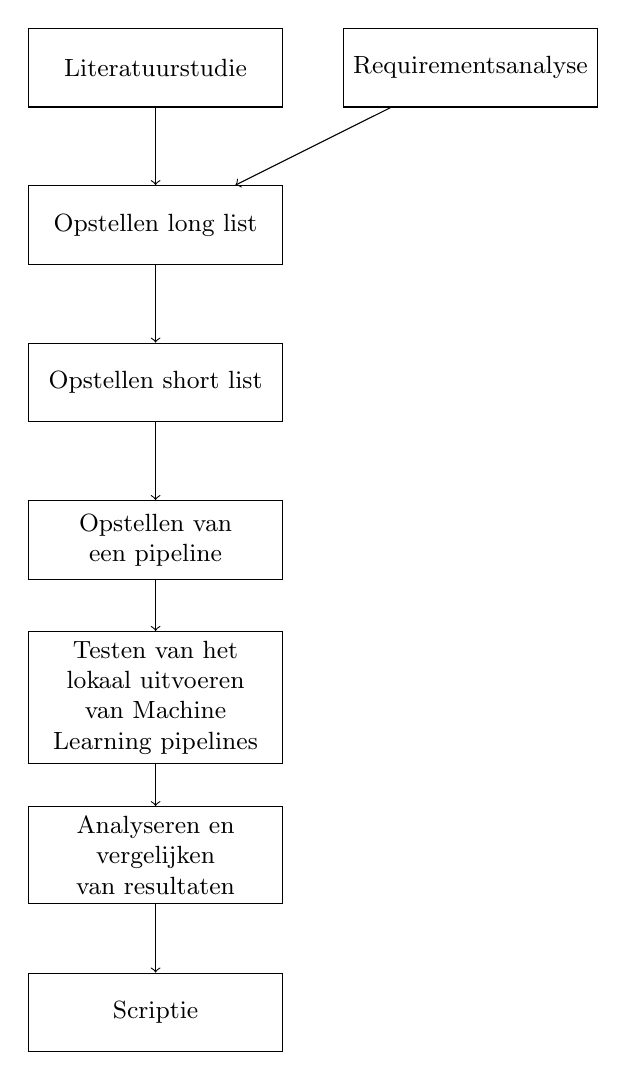
\begin{tikzpicture}[node distance=2cm, every node/.style={font=\small}]
  \node (pro0) [rectangle, draw, minimum width=3cm, minimum height=1cm, text centered, text width=3cm] {Literatuurstudie};
  \node (pro8) [rectangle, draw, minimum width=3cm, minimum height=1cm, text centered, text width=3cm, right of=pro0, xshift=2cm] {Requirements\-analyse};
  \node (pro1) [rectangle, draw, minimum width=3cm, minimum height=1cm, text centered, text width=3cm,below of=pro0] {Opstellen long list};
  \node (pro3) [rectangle, draw, minimum width=3cm, minimum height=1cm, text centered, text width=3cm, below of=pro1] {Opstellen short list};
  \node (pro4) [rectangle, draw, minimum width=3cm, minimum height=1cm, text centered, text width=3cm, below of=pro3] {Opstellen van een pipeline};
  \node (pro5) [rectangle, draw, minimum width=3cm, minimum height=1cm, text centered, text width=3cm, below of=pro4] {Testen van het lokaal uitvoeren van Machine Learning pipelines};
  \node (pro6) [rectangle, draw, minimum width=3cm, minimum height=1cm, text centered, text width=3cm, below of=pro5] {Analyseren en vergelijken van resultaten};
  \node (pro7) [rectangle, draw, minimum width=3cm, minimum height=1cm, text centered, text width=3cm, below of=pro6] {Scriptie};

  \draw [->] (pro0) -- (pro1);
  \draw [->] (pro1) -- (pro3);
  \draw [->] (pro3) -- (pro4);
  \draw [->] (pro4) -- (pro5);
  \draw [->] (pro5) -- (pro6);
  \draw [->] (pro6) -- (pro7);
  \draw [->] (pro8) -- (pro1);
\end{tikzpicture}


%Hier beschrijf je hoe je van plan bent het onderzoek te voeren. Welke onderzoekstechniek ga je toepassen om elk van je onderzoeksvragen te beantwoorden? Gebruik je hiervoor literatuurstudie, interviews met belanghebbenden (bv.~voor requirements-analyse), experimenten, simulaties, vergelijkende studie, risico-analyse, PoC, \ldots?

%Valt je onderwerp onder één van de typische soorten bachelorproeven die besproken zijn in de lessen Research Methods (bv.\ vergelijkende studie of risico-analyse)? Zorg er dan ook voor dat we duidelijk de verschillende stappen terug vinden die we verwachten in dit soort onderzoek!

%Vermijd onderzoekstechnieken die geen objectieve, meetbare resultaten kunnen opleveren. Enquêtes, bijvoorbeeld, zijn voor een bachelorproef informatica meestal \textbf{niet geschikt}. De antwoorden zijn eerder meningen dan feiten en in de praktijk blijkt het ook bijzonder moeilijk om voldoende respondenten te vinden. Studenten die een enquête willen voeren, hebben meestal ook geen goede definitie van de populatie, waardoor ook niet kan aangetoond worden dat eventuele resultaten representatief zijn.

%Uit dit onderdeel moet duidelijk naar voor komen dat je bachelorproef ook technisch voldoen\-de diepgang zal bevatten. Het zou niet kloppen als een bachelorproef informatica ook door bv.\ een student marketing zou kunnen uitgevoerd worden.

%Je beschrijft ook al welke tools (hardware, software, diensten, \ldots) je denkt hiervoor te gebruiken of te ontwikkelen.

%Probeer ook een tijdschatting te maken. Hoe lang zal je met elke fase van je onderzoek bezig zijn en wat zijn de concrete \emph{deliverables} in elke fase?

%---------- Verwachte resultaten ----------------------------------------------
\section{Verwacht resultaat, conclusie}%
\label{sec:verwachte_resultaten}
Dit onderzoek heeft als doel om personen in het vakgebied Machine Learning Operations te voorzien van een duidelijke aanbeveling voor het lokaal uitvoeren van Machine Learning pipelines. Het verwachte resultaat omvat een overzicht van beschikbare frameworks en bibliotheken, met de identificatie van de meest veelbelovende opties op basis van criteria zoals installatiegemak, prestaties en compatibiliteit. Het onderzoek zal praktische testresultaten presenteren die laten zien hoe deze geselecteerde tools presteren in de praktijk. Een conclusie en aanbeveling zullen worden geformuleerd op basis van deze resultaten, samen met beknopte praktische richtlijnen voor het gebruik van het aanbevolen framework of bibliotheek. Bovendien zal het onderzoek inzicht verschaffen in de uitdagingen en mogelijke obstakels bij het lokaal uitvoeren van Machine Learning pipelines.

%Hier beschrijf je welke resultaten je verwacht. Als je metingen en simulaties uitvoert, kan je hier al mock-ups maken van de grafieken samen met de verwachte conclusies. Benoem zeker al je assen en de onderdelen van de grafiek die je gaat gebruiken. Dit zorgt ervoor dat je concreet weet welk soort data je moet verzamelen en hoe je die moet meten.

%Wat heeft de doelgroep van je onderzoek aan het resultaat? Op welke manier zorgt jouw bachelorproef voor een meerwaarde?

%Hier beschrijf je wat je verwacht uit je onderzoek, met de motivatie waarom. Het is \textbf{niet} erg indien uit je onderzoek andere resultaten en conclusies vloeien dan dat je hier beschrijft: het is dan juist interessant om te onderzoeken waarom jouw hypothesen niet overeenkomen met de resultaten.

\printbibliography[heading=bibintoc]

\end{document}